\documentclass{exam}
\usepackage[spanish,activeacute]{babel}
\usepackage[utf8]{inputenc}
\usepackage[T1]{fontenc}
\usepackage[newcommands]{ragged2e}

\usepackage{
    amsmath,
    amssymb,
    eso-pic,
    float,
    graphicx,
    lmodern,
    wrapfig,
    tabularx,
    multicol,
    multirow,
    color,
    colortbl,
    lastpage,
    titlesec,
    sectsty
}

\definecolor{azul}{RGB}{33,127,190}
\sectionfont{\color{azul}}
\subsectionfont{\color{azul}}
\renewcommand{\familydefault}{\sfdefault}

\footer{}{\thepage}{}

\makeatother

\title{\LARGE\color{azul}\textbf{ICI 202 Programaci\'on 2 - Ejercicio sumativo 07 }}
\author{\normalsize \color{gray}{Prof.} \color{black}{\textbf{Ismael Figueroa, Eduardo Godoy}}}
\date{\normalsize \em \today}

\begin{document}

\AddToShipoutPictureBG*{%
  \AtPageUpperLeft{\raisebox{-\height}{
\includegraphics[scale=.95]{base/header.png}}}}

\maketitle

\begin{multicols}{2} \begin{flushleft} \textbf{Nombre:} \\ \vspace*{2mm} \textbf{Rut:} \\ \vspace*{2mm} \textbf{Paralelo:} \end{flushleft} \begin{center} \begin{table}[H] \begin{tabular}{p{4cm}|p{3cm}|} \arrayrulecolor{gray!50}\cline{2-2} ~ & {\em {\scriptsize \color{gray!50}{Puntaje:}}} \\ & ~ \\ ~ & \textbf{Nota:} \\ & ~ \\ \arrayrulecolor{gray!50}\cline{2-2} \end{tabular} \end{table} \end{center} \end{multicols}

\vspace*{-18mm}
\noindent
\textbf{\\Instrucciones:}
\begin{itemize}
    \item[-] El puntaje m\'aximo  es 100 puntos.
    \item[-] Tiempo m\'aximo: 90 minutos.
    \item[-] El trabajo es \underline{\textbf{individual}}. Cualquier intento de copia, ser\'a sancionado seg\'un dicta el reglamento de la carrera.
    \item[-] Se debe subir al aula virtual un archivo comprimido con el siguiente formato \\ Ej07\_<NombreApellidoEstudiante\_rut\_paralelo>.zip, dentro de el deben estar los c\'odigos fuentes requeridos.
\end{itemize}

\noindent
\textbf{Resultados de aprendizaje a evaluar:}
\begin{enumerate}
  \item Resoluci\'on de problemas utilizando Lenguaje Java.
  \item Implementación de Interfaces.
  \item Uso de Polimorfismo
\end{enumerate}
\vspace{2mm}

\noindent
\textbf{Contenido:} Este Ejercicios eval\'ua los siguientes temas:

\vspace{-2mm}
\begin{table}[H]
\begin{tabular}{
    !{\color{gray!50}\vrule}l
    !{\color{gray!50}\vrule}c
    !{\color{gray!50}\vrule}c
    !{\color{gray!50}\vrule}} \arrayrulecolor{gray!50} \hline
    \multicolumn{1}{!{\color{gray!50}\vrule}c}{\multirow{2}{*}{\textbf{
        Tema
    }}} &
    \multicolumn{2}{!{\color{gray!50}\vrule}c!{\color{gray!50}\vrule}}{\textbf{
        Puntajes
    }} \\ \arrayrulecolor{gray!50}\cline{2-3} &
    \multicolumn{1}{!{\color{gray!50}\vrule}c!{\color{gray!50}\vrule}}{\textbf{
        Total
    }} &
    \multicolumn{1}{c!{\color{gray!50}\vrule}}{\textbf{
        Obtenido
    }} \\ \arrayrulecolor{gray!50} \hline
    Creaci\'on de Clase con atributos.
    & \multicolumn{1}{!{\color{gray!50}\vrule}c!{\color{gray!50}\vrule}}{\textbf{
        10 pts.
    }} & \\ \arrayrulecolor{gray!50} \hline
    Implementaci\'on de m\'etodos (comportamientos) asociados y correcto funcionamiento.
    & \multicolumn{1}{!{\color{gray!50}\vrule}c!{\color{gray!50}\vrule}}{\textbf{
        60 pts.
    }} & \\ \arrayrulecolor{gray!50} \hline
    Implementar clase instanciadora con m\'etodo main.
    & \multicolumn{1}{!{\color{gray!50}\vrule}c!{\color{gray!50}\vrule}}{\textbf{
        20 pts.
    }} & \\ \arrayrulecolor{gray!50} \hline
    Cumple con el formato y compilaci\'on correcta
    & \multicolumn{1}{!{\color{gray!50}\vrule}c!{\color{gray!50}\vrule}}{\textbf{
        10 pts.
    }} & \\ \arrayrulecolor{gray!50} \hline

\end{tabular}
\end{table}

\vspace{-7mm}
\newpage
\section{\textbf{Programaci\'on en Java (100 pts)}}
\noindent
\textbf{Plantamiento de problema: }

\begin{questions}

  \begin{itemize}
    \item  Se requiere crear un programa que permita visualizar un proceso de partidos clasificatorios al mundial de Qatar 2018.  Se entiende que una persona perteneciente al proceso de clasificación debe
    realizar las siguientes actividades: concentrarse, entrenar, viajar y jugar el partido. PAra más detalle se presenta la Figura 1 modelo de clases.
\item Adicionalmente se requiere que cada clase identificada en el modelo contenga los m\'etodos requeridos e implementados seg\un la interface de referencia, el detalle de la implementaci\'on de
cada m\'etodo se detalla a continuaci\'on:

\begin{enumerate}
  \item Futbolista
  \begin{itemize}
    \item Crear darEntrevista() que imprima en pantalla: Da una Entrevista (Clase Futbolista)
    \item Implementar concentrarse() que imprima en pantalla: Concentrarse (Clase Futbolista)
    \item Implementar viajar() que imprima en pantalla: Viajar (Clase Futbolista)
    \item Implementar entrenar() que imprima en pantalla: Realiza un entrenamiento (Clase Futbolista)
    \item Implementar jugarPartido() que imprima en pantalla: Juega un Partido (Clase Futbolista)
  \end{itemize}
  \item Entrenador
  \begin{itemize}
    \item Crear planificarEntrenamiento() que imprima en pantalla: Planificar un Entrenamiento
    \item Implementar concentrarse() que imprima en pantalla: Concentrarse (Clase Entrenador)
    \item Implementar viajar() que imprima en pantalla: Viajar (Clase Futbolista)
    \item Implementar entrenar() que imprima en pantalla: Entrenar (Clase Entrenador)
    \item Implementar jugarPartido() que imprima en pantalla: Asiste al Partido de Fútbol (Clase Entrenador)
  \end{itemize}
  \item Asistente
  \begin{itemize}
    \item Crear darAsistencia() que imprima en pantalla: Da una Asistencia medica
    \item Implementar concentrarse() que imprima en pantalla: Concentrarse (Clase Asistente)
    \item Implementar viajar() que imprima en pantalla: Viajar (Clase Asistente)
    \item Implementar entrenar() que imprima en pantalla: Da una Asistencia medica en el entrenamiento (Clase Asistente)
    \item Implementar jugarPartido() que imprima en pantalla: Asiste al Partido de Fútbol y apoya fisicamente a los deportistas (Clase Asistente)
  \end{itemize}
\end{enumerate}

\item Tambi\'en se debe ejecutar la clase SeleccionMain.java para validar la implementaci\'on realizada.



    \newpage
    \begin{figure}
      \centering
        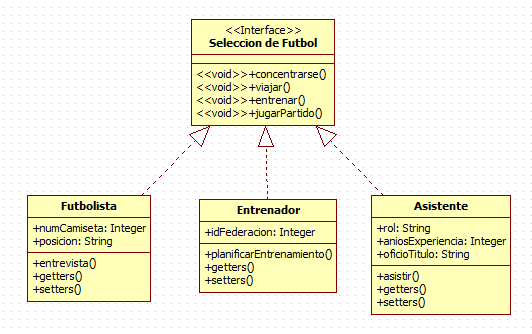
\includegraphics{base/modeloSeleccion.png}
      \caption{Modelo de Clases}
      \label{fig:ejemplo}
    \end{figure}

\item Objetivo del trabajo:

  \begin{enumerate}
    \item \emph{(10pts)} Crear la interface y definir en ella los m\'etodos requeridos seg\'un  modelo y detalle anterior.
    \item \emph{(60pts)} Codificar las clases que implementan dicha interfaces y el detalle de cada m\'etodo tambi\'en implementado.
    \item \emph{(20pts)} Considera la clase entregada SeleccionMain.java para ejecutar el programa requerido.
  \end{enumerate}

  \begin{itemize}
    \item Salida Esperada del programa:\\ \\
Concentrarse (Clase Entrenador)\\
Concentrarse (Clase Futbolista)\\
Concentrarse (Clase Asistente)\\
Entrenar (Clase Entrenador)\\
Realiza un entrenamiento (Clase Futbolista)\\
Da una Asistencia medica en el entrenamiento (Clase Asistente)\\
Viajar (Clase Entrenador)\\
Viajar (Clase Futbolista)\\
Viajar (Clase Asistente)\\
Asiste al Partido de Fútbol (Clase Entrenador)\\
Juega un Partido (Clase Futbolista)\\
Asiste al Partido de Fútbol y apoya fisicamente a los deportistas (Clase Asistente)\\
Planificar un Entrenamiento\\
Da una Entrevista (Clase Futbolista)\\
Da una Asistencia medica\\
  \end{itemize}
\end{itemize}
\end{questions}

\begin{table}[H]
\centering
\begin{tabular}{
!{\color{gray!50}\vrule}p{3.9cm}
!{\color{gray!50}\vrule}p{3.6cm}
!{\color{gray!50}\vrule}p{3.6cm}
!{\color{gray!50}\vrule}p{3.6cm}
!{\color{gray!50}\vrule}} \arrayrulecolor{gray!50} \hline
    \multicolumn{4}{!{\color{gray!50}\vrule}c!{\color{gray!50}\vrule}}{\textbf{?`C\'omo ser{\'e} evaluado en este trabajo?}} \\ \arrayrulecolor{gray!50} \hline
    \textbf{\'Item} & \textbf{Logrado} & \textbf{Suficiente} & \textbf{No Logrado}\\ \arrayrulecolor{gray!50} \hline
  \newline Herencia y Polimorfismo, Creaci\'on de Clase con atributos. &
  \newline  Aplica de forma correcta 30\%  ... &
  \newline Aplica parcialmente con menos de 2 errores 20\% ... &
    \newline Aplica de forma incorrecta con 3 errores o m\'as 0-9\%\\ \arrayrulecolor{gray!50} \hline
    \newline  Implementaci\'on de m\'etodos (comportamientos) asociados y correcto funcionamiento. &
    \newline  Aplica de forma correcta 30\%  ... &
    \newline Aplica parcialmente con menos de 2 errores 20\%... &
    \newline Aplica de forma incorrecta con 3 errores o m\'as 0-8\%\\ \arrayrulecolor{gray!50} \hline
  \newline  Implementar clase instanciadora con m\'etodo main y crea instancias de objetos. &
  \newline  Aplica de forma correcta 30\%... &
    \newline  Aplica parcialmente con menos de 2 errores 15\%... &
    \newline Aplica de forma incorrecta con 3 errores o m\'as 0-9\%\\ \arrayrulecolor{gray!50} \hline
    \newline  Cumple con el formato y compilaci\'on correcta &
    \newline  Aplica de forma correcta 10\% ... &
    \newline Aplica parcialmente con menos de x errores 5\%... &
    \newline Aplica de forma incorrecta con x errores o m\'as 0-4\%\\ \arrayrulecolor{gray!50} \hline
    Total de la secci\'on &  100\% & 60\% & 0-30\%\\ \arrayrulecolor{gray!50} \hline
\end{tabular}
\label{tbl:1}
\end{table}
\vspace{-5mm}
\textbf{Nota:} En caso de que el {\'i}tem no est{\'e} presente, tiene ponderaci{\'o}n cero.

\end{document}
